%!TEX root = ceres-solver.tex
\chapter{Modeling}
\label{chapter:api}
\section{\texttt{CostFunction}}
Given parameter blocks $\left[x_{i_1}, \hdots , x_{i_k}\right]$, a \texttt{CostFunction} is responsible for computing
a vector of residuals and if asked a vector of Jacobian matrices, i.e., given $\left[x_{i_1}, \hdots , x_{i_k}\right]$, compute the vector $f_i\left(x_{i_1},\hdots,x_{k_i}\right)$ and the matrices
\begin{equation}
J_{ij} = \frac{\partial}{\partial x_{i_j}}f_i\left(x_{i_1},\hdots,x_{k_i}\right),\quad \forall j = i_1,\hdots, i_k
\end{equation}
\begin{minted}{c++}
class CostFunction {
 public:
  virtual bool Evaluate(double const* const* parameters,
                        double* residuals,
                        double** jacobians) = 0;
  const vector<int16>& parameter_block_sizes();
  int num_residuals() const;

 protected:
  vector<int16>* mutable_parameter_block_sizes();
  void set_num_residuals(int num_residuals);
};
\end{minted}

The signature of the function (number and sizes of input parameter blocks and number of outputs)
is stored in \texttt{parameter\_block\_sizes\_} and \texttt{num\_residuals\_} respectively. User
code inheriting from this class is expected to set these two members with the
corresponding accessors. This information will be verified by the Problem
when added with \texttt{Problem::AddResidualBlock}.

The most important method here is \texttt{Evaluate}. It implements the residual and Jacobian computation.

\texttt{parameters}  is an array of pointers to arrays containing the various parameter blocks. parameters has the same number of elements as parameter\_block\_sizes\_.  Parameter blocks are in the same order as parameter\_block\_sizes\_.


\texttt{residuals} is an array of size \texttt{num\_residuals\_}.


\texttt{jacobians} is an array of size \texttt{parameter\_block\_sizes\_} containing pointers to storage for Jacobian matrices corresponding to each parameter block. The Jacobian matrices are in the same order as \texttt{parameter\_block\_sizes\_}. \texttt{jacobians[i]} is an array that contains \texttt{num\_residuals\_} $\times$ \texttt{parameter\_block\_sizes\_[i]} elements. Each Jacobian matrix is stored in row-major order, i.e.,

\begin{equation}
\texttt{jacobians[i][r * parameter\_block\_size\_[i] + c]} =
%\frac{\partial}{\partial x_{ic}}  f_{r}\left(x_{1},\hdots, x_{k}\right)
\frac{\partial \texttt{residual[r]}}{\partial \texttt{parameters[i][c]}}
\end{equation}

If \texttt{jacobians} is \texttt{NULL}, then no derivatives are returned; this is the case when computing cost only. If \texttt{jacobians[i]} is \texttt{NULL}, then the Jacobian matrix corresponding to the $i^{\textrm{th}}$ parameter block must not be returned, this is the case when the a parameter block is marked constant.

\section{\texttt{SizedCostFunction}}
If the size of the parameter blocks and the size of the residual vector is known at compile time (this is the common case), Ceres provides \texttt{SizedCostFunction}, where these values can be specified as template parameters.
\begin{minted}{c++}
template<int kNumResiduals,
         int N0 = 0, int N1 = 0, int N2 = 0, int N3 = 0, int N4 = 0, int N5 = 0>
class SizedCostFunction : public CostFunction {
 public:
  virtual bool Evaluate(double const* const* parameters,
                        double* residuals,
                        double** jacobians) = 0;
};
\end{minted}
In this case the user only needs to implement the \texttt{Evaluate} method.

\section{\texttt{AutoDiffCostFunction}}
But even defining the \texttt{SizedCostFunction} can be a tedious affair if complicated derivative computations are involved. To this end Ceres provides automatic differentiation.

To get an auto differentiated cost function, you must define a class with a
 templated \texttt{operator()} (a functor) that computes the cost function in terms of
 the template parameter \texttt{T}. The autodiff framework substitutes appropriate
 \texttt{Jet} objects for T in order to compute the derivative when necessary, but
 this is hidden, and you should write the function as if T were a scalar type
 (e.g. a double-precision floating point number).

 The function must write the computed value in the last argument (the only
 non-\texttt{const} one) and return true to indicate success.

 For example, consider a scalar error $e = k - x^\top y$, where both $x$ and $y$ are
 two-dimensional vector parameters  and $k$ is a constant. The form of this error, which is the
 difference between a constant and an expression, is a common pattern in least
 squares problems. For example, the value $x^\top y$ might be the model expectation
 for a series of measurements, where there is an instance of the cost function
 for each measurement $k$.

 The actual cost added to the total problem is $e^2$, or $(k - x^\top y)^2$; however,
 the squaring is implicitly done by the optimization framework.

 To write an auto-differentiable cost function for the above model, first
 define the object
\begin{minted}{c++}
class MyScalarCostFunction {
  MyScalarCostFunction(double k): k_(k) {}
  template <typename T>
  bool operator()(const T* const x , const T* const y, T* e) const {
    e[0] = T(k_) - x[0] * y[0] + x[1] * y[1]
     return true;
  }

 private:
  double k_;
};
\end{minted}

Note that in the declaration of \texttt{operator()} the input parameters \texttt{x} and \texttt{y} come
 first, and are passed as const pointers to arrays of \texttt{T}. If there were three
 input parameters, then the third input parameter would come after \texttt{y}. The
 output is always the last parameter, and is also a pointer to an array. In
 the example above, \texttt{e} is a scalar, so only \texttt{e[0]} is set.

 Then given this class definition, the auto differentiated cost function for
 it can be constructed as follows.

\begin{minted}{c++}
CostFunction* cost_function
    = new AutoDiffCostFunction<MyScalarCostFunction, 1, 2, 2>(
        new MyScalarCostFunction(1.0));              ^  ^  ^
                                                     |  |  |
                         Dimension of residual ------+  |  |
                         Dimension of x ----------------+  |
                         Dimension of y -------------------+
\end{minted}

In this example, there is usually an instance for each measurement of k.

In the instantiation above, the template parameters following
 \texttt{MyScalarCostFunction}, \texttt{<1, 2, 2>} describe the functor as computing a
 1-dimensional output from two arguments, both 2-dimensional.

 The framework can currently accommodate cost functions of up to 6 independent
 variables, and there is no limit on the dimensionality of each of them.

 \textbf{WARNING 1} Since the functor will get instantiated with different types for
 \texttt{T}, you must convert from other numeric types to \texttt{T} before mixing
 computations with other variables of type \texttt{T}. In the example above, this is
 seen where instead of using \texttt{k\_} directly, \texttt{k\_} is wrapped with \texttt{T(k\_)}.

 \textbf{WARNING 2} A common beginner's error when first using \texttt{AutoDiffCostFunction} is to get the sizing wrong. In particular, there is a tendency to
 set the template parameters to (dimension of residual, number of parameters)
 instead of passing a dimension parameter for {\em every parameter block}. In the
 example above, that would be \texttt{<MyScalarCostFunction, 1, 2>}, which is missing
 the 2 as the last template argument.

\subsection{Theory \& Implementation}
TBD

\section{\texttt{NumericDiffCostFunction}}
To get a numerically differentiated cost function, define a subclass of
\texttt{CostFunction} such that the \texttt{Evaluate} function ignores the jacobian
parameter. The numeric differentiation wrapper will fill in the jacobians array
 if necessary by repeatedly calling the \texttt{Evaluate} method with
small changes to the appropriate parameters, and computing the slope. For
performance, the numeric differentiation wrapper class is templated on the
concrete cost function, even though it could be implemented only in terms of
the virtual \texttt{CostFunction} interface.
\begin{minted}{c++}
template <typename CostFunctionNoJacobian,
          NumericDiffMethod method = CENTRAL, int M = 0,
          int N0 = 0, int N1 = 0, int N2 = 0, int N3 = 0, int N4 = 0, int N5 = 0>
class NumericDiffCostFunction
    : public SizedCostFunction<M, N0, N1, N2, N3, N4, N5> {
};
\end{minted}

The numerically differentiated version of a cost function for a cost function
can be constructed as follows:
\begin{minted}{c++}
CostFunction* cost_function
    = new NumericDiffCostFunction<MyCostFunction, CENTRAL, 1, 4, 8>(
        new MyCostFunction(...), TAKE_OWNERSHIP);
\end{minted}
where \texttt{MyCostFunction} has 1 residual and 2 parameter blocks with sizes 4 and 8
respectively. Look at the tests for a more detailed example.

The central difference method is considerably more accurate at the cost of
twice as many function evaluations than forward difference. Consider using
central differences begin with, and only after that works, trying forward
difference to improve performance.

\section{\texttt{LossFunction}}
 For least squares problems where the minimization may encounter
 input terms that contain outliers, that is, completely bogus
 measurements, it is important to use a loss function that reduces
 their influence.

 Consider a structure from motion problem. The unknowns are 3D
 points and camera parameters, and the measurements are image
 coordinates describing the expected reprojected position for a
 point in a camera. For example, we want to model the geometry of a
 street scene with fire hydrants and cars, observed by a moving
 camera with unknown parameters, and the only 3D points we care
 about are the pointy tippy-tops of the fire hydrants. Our magic
 image processing algorithm, which is responsible for producing the
 measurements that are input to Ceres, has found and matched all
 such tippy-tops in all image frames, except that in one of the
 frame it mistook a car's headlight for a hydrant. If we didn't do
 anything special  the
 residual for the erroneous measurement will result in the
 entire solution getting pulled away from the optimum to reduce
 the large error that would otherwise be attributed to the wrong
 measurement.

 Using a robust loss function, the cost for large residuals is
 reduced. In the example above, this leads to outlier terms getting
 down-weighted so they do not overly influence the final solution.

\begin{minted}{c++}
class LossFunction {
 public:
  virtual void Evaluate(double s, double out[3]) const = 0;
};
\end{minted}

The key method is \texttt{Evaluate}, which given a non-negative scalar \texttt{s}, computes
\begin{align}
	\texttt{out} = \begin{bmatrix}\rho(s), & \rho'(s), & \rho''(s)\end{bmatrix}
\end{align}

Here the convention is that the contribution of a term to the cost function is given by $\frac{1}{2}\rho(s)$,  where $s = \|f_i\|^2$. Calling the method with a negative value of $s$ is an error and the implementations are not required to handle that case.

Most sane choices of $\rho$ satisfy:
\begin{align}
   \rho(0) &= 0\\
   \rho'(0) &= 1\\
   \rho'(s) &< 1 \text{ in the outlier region}\\
   \rho''(s) &< 0 \text{ in the outlier region}
\end{align}
so that they mimic the squared cost for small residuals.

\subsection{Scaling}
Given one robustifier $\rho(s)$
 one can change the length scale at which robustification takes
 place, by adding a scale factor $a > 0$ which gives us $\rho(s,a) = a^2 \rho(s / a^2)$ and the first and second derivatives as $\rho'(s / a^2)$ and   $(1 / a^2) \rho''(s / a^2)$ respectively.


\begin{figure}[hbt]
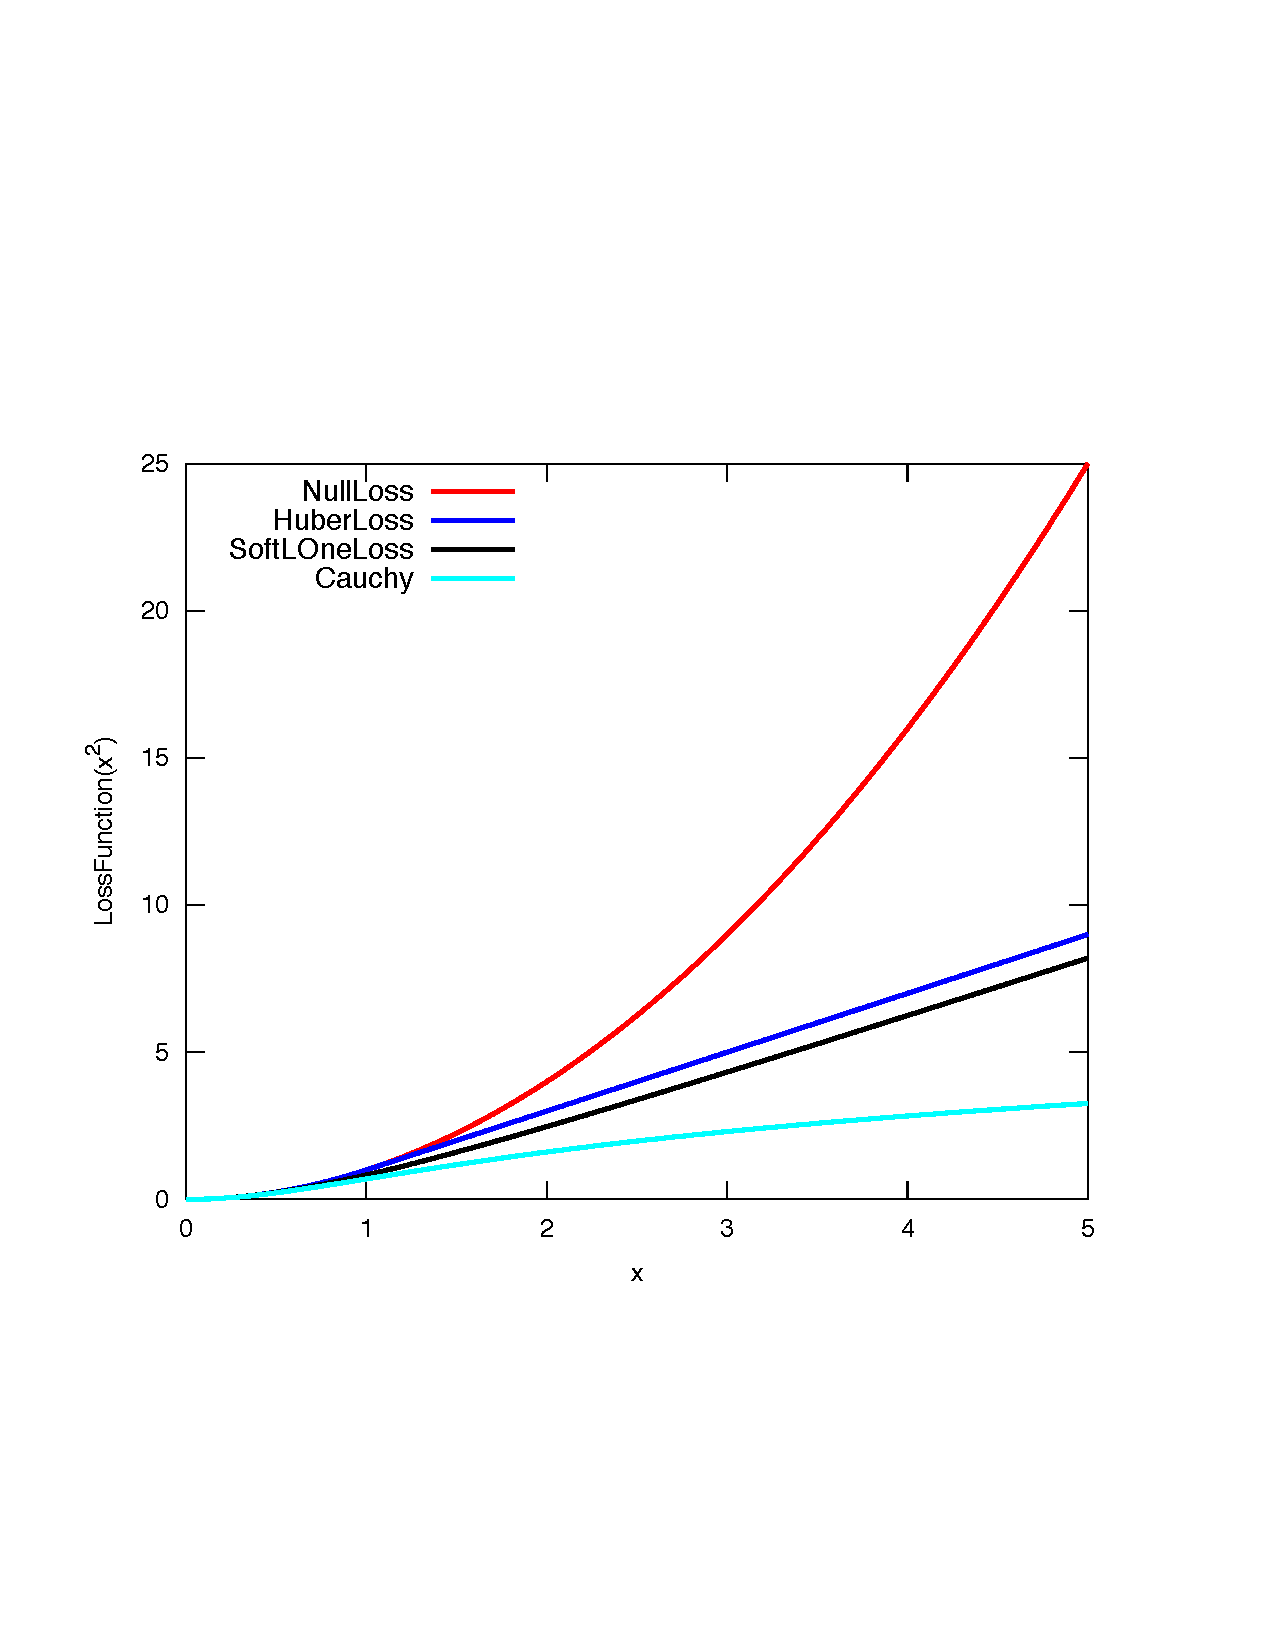
\includegraphics[width=\textwidth]{loss.pdf}
\caption{Shape of the various common loss functions.}
\label{fig:loss}
\end{figure}


The reason for the appearance of squaring is that $a$ is in the units of the residual vector norm whereas $s$ is a squared norm. For applications it is more convenient to specify $a$ than
its square.

Here are some common loss functions implemented in Ceres. For simplicity we described their unscaled versions. Figure~\ref{fig:loss} illustrates their shape graphically.

\begin{align}
		\rho(s)&=s \tag{\texttt{NullLoss}}\\
		\rho(s) &= \begin{cases}
		       s & s \le 1\\
		       2 \sqrt{s} - 1 & s > 1
	           \end{cases} \tag{\texttt{HuberLoss}}\\
		\rho(s) &= 2 (\sqrt{1+s} - 1) \tag{\texttt{SoftLOneLoss}}\\
		\rho(s) &= \log(1 + s) \tag{\texttt{CauchyLoss}}
\end{align}

Ceres includes a number of other loss functions, the descriptions and
documentation for which can be found in \texttt{loss\_function.h}.

\subsection{Theory \& Implementation}
Let us consider a problem with a single problem and a single parameter
block.
\begin{align}
\min_x \frac{1}{2}\rho(f^2(x))
\end{align}

Then, the robustified gradient and the Gauss-Newton Hessian are
\begin{align}
	g(x) &= \rho'J^\top(x)f(x)\\
	H(x) &= J^\top(x)\left(\rho' + 2 \rho''f(x)f^\top(x)\right)J(x) 
\end{align}
where the terms involving the second derivatives of $f(x)$ have been ignored. Note that $H(x)$ is indefinite if $\rho''f(x)^\top f(x) + \frac{1}{2}\rho' < 0$. If this is not the case, then its possible to re-weight the residual and the Jacobian matrix such that the corresponding linear least squares problem for the robustified Gauss-Newton step. 


Let $\alpha$ be a root of 
\begin{equation}
	\frac{1}{2}\alpha^2 - \alpha - \frac{\rho''}{\rho'}\|f(x)\|^2 = 0.
\end{equation}
Then, define the rescaled residual and Jacobian as
\begin{align}
	\tilde{f}(x) &= \frac{\sqrt{\rho'}}{1 - \alpha} f(x)\\
	\tilde{J}(x) &= \sqrt{\rho'}\left(1 - \alpha \frac{f(x)f^\top(x)}{\left\|f(x)\right\|^2} \right)J(x)
\end{align}
In the case $2 \rho''\left\|f(x)\right\|^2 + \rho' \lesssim 0$, we limit $\alpha \le 1- \epsilon$ for some small $\epsilon$. For more details see Triggs et al~\cite{triggs-etal-1999}.

With this simple rescaling, one can use any Jacobian based non-linear least squares algorithm to robustifed non-linear least squares problems.

\section{\texttt{LocalParameterization}}
Sometimes the parameters $x$ can overparameterize a problem. In
that case it is desirable to choose a parameterization to remove
the null directions of the cost. More generally, if $x$ lies on a
manifold of a smaller dimension than the ambient space that it is
embedded in, then it is numerically and computationally more
effective to optimize it using a parameterization that lives in
the tangent space of that manifold at each point.

For example, a sphere in three dimensions is a two dimensional
manifold, embedded in a three dimensional space. At each point on
the sphere, the plane tangent to it defines a two dimensional
tangent space. For a cost function defined on this sphere, given a
point $x$, moving in the direction normal to the sphere at that
point is not useful. Thus a better way to parameterize a point on
a sphere is to optimize over two dimensional vector $\Delta x$ in the
tangent space at the point on the sphere point and then "move" to
the point $x + \Delta x$, where the move operation involves projecting
back onto the sphere. Doing so removes a redundant dimension from
the optimization, making it numerically more robust and efficient.

More generally we can define a function
\begin{equation}
  x' = \boxplus(x, \Delta x),
\end{equation}
where $x'$ has the same size as $x$, and $\Delta x$ is of size less
than or equal to $x$. The function $\boxplus$, generalizes the
definition of vector addition. Thus it satisfies the identity
\begin{equation}
  \boxplus(x, 0) = x,\quad \forall x.
\end{equation}

Instances of \texttt{LocalParameterization} implement the $\boxplus$ operation and its derivative with respect to $\Delta x$ at $\Delta x = 0$.

\begin{minted}{c++}
class LocalParameterization {
 public:
  virtual ~LocalParameterization() {}
  virtual bool Plus(const double* x,
                    const double* delta,
                    double* x_plus_delta) const = 0;
  virtual bool ComputeJacobian(const double* x, double* jacobian) const = 0;
  virtual int GlobalSize() const = 0;
  virtual int LocalSize() const = 0;
};
\end{minted}

\texttt{GlobalSize} is the dimension of the ambient space in which the parameter block $x$ lives. \texttt{LocalSize} is the size of the tangent space that $\Delta x$ lives in. \texttt{Plus} implements $\boxplus(x,\Delta x)$ and $\texttt{ComputeJacobian}$ computes the Jacobian matrix
\begin{equation}
	J = \left . \frac{\partial }{\partial \Delta x} \boxplus(x,\Delta x)\right|_{\Delta x = 0}
\end{equation}
in row major form.

A trivial version of $\boxplus$ is when delta is of the same size as $x$
and

\begin{equation}
  \boxplus(x, \Delta x) = x + \Delta x
\end{equation}

A more interesting case if $x$ is a two dimensional vector, and the
user wishes to hold the first coordinate constant. Then, $\Delta x$ is a
scalar and $\boxplus$ is defined as

\begin{equation}
  \boxplus(x, \Delta x) = x + \left[ \begin{array}{c} 0 \\ 1
                                  \end{array} \right]        \Delta x
\end{equation}

\texttt{SubsetParameterization} generalizes this construction to hold any part of a parameter block constant.


Another example that occurs commonly in Structure from Motion problems
is when camera rotations are parameterized using a quaternion. There,
it is useful only to make updates orthogonal to that 4-vector defining
the quaternion. One way to do this is to let $\Delta x$ be a 3
dimensional vector and define $\boxplus$ to be

\begin{equation}
  \boxplus(x, \Delta x) =
\left[
\cos(|\Delta x|), \frac{\sin\left(|\Delta x|\right)}{|\Delta x|} \Delta x
\right] * x
\label{eq:quaternion}
\end{equation}
The multiplication between the two 4-vectors on the right hand
side is the standard quaternion product. \texttt{QuaternionParameterization} is an implementation of~\eqref{eq:quaternion}.

\clearpage

\section{\texttt{Problem}}
\begin{minted}{c++}
class Problem {
 public:
  struct Options {
    Options();
    Ownership cost_function_ownership;
    Ownership loss_function_ownership;
    Ownership local_parameterization_ownership;
  };

  Problem();
  explicit Problem(const Options& options);
  ~Problem();

  ResidualBlockId AddResidualBlock(CostFunction* cost_function,
                                   LossFunction* loss_function,
                                   const vector<double*>& parameter_blocks);

  void AddParameterBlock(double* values, int size);
  void AddParameterBlock(double* values,
                         int size,
                         LocalParameterization* local_parameterization);

  void SetParameterBlockConstant(double* values);
  void SetParameterBlockVariable(double* values);
  void SetParameterization(double* values,
                           LocalParameterization* local_parameterization);

  int NumParameterBlocks() const;
  int NumParameters() const;
  int NumResidualBlocks() const;
  int NumResiduals() const;
};
\end{minted}

The \texttt{Problem} objects holds the robustified non-linear least squares problem~\eqref{eq:ceresproblem}. To create a least squares problem, use the \texttt{Problem::AddResidualBlock} and \texttt{Problem::AddParameterBlock} methods.

For example a problem containing 3 parameter blocks of sizes 3, 4 and 5
respectively and two residual blocks  of size 2 and 6:

\begin{minted}{c++}
double x1[] = { 1.0, 2.0, 3.0 };
double x2[] = { 1.0, 2.0, 3.0, 5.0 };
double x3[] = { 1.0, 2.0, 3.0, 6.0, 7.0 };

Problem problem;
problem.AddResidualBlock(new MyUnaryCostFunction(...), x1);
problem.AddResidualBlock(new MyBinaryCostFunction(...), x2, x3);
\end{minted}


\texttt{AddResidualBlock} as the name implies, adds a residual block to the problem. It adds a cost function, an optional loss function, and connects the cost function to a set of parameter blocks.

The cost
   function carries with it information about the sizes of the
   parameter blocks it expects. The function checks that these match
   the sizes of the parameter blocks listed in \texttt{parameter\_blocks}. The
   program aborts if a mismatch is detected. \texttt{loss\_function} can be
   \texttt{NULL}, in which case the cost of the term is just the squared norm
   of the residuals.

  The user has the option of explicitly adding the parameter blocks
  using \texttt{AddParameterBlock}. This causes additional correctness
  checking; however, \texttt{AddResidualBlock} implicitly adds the parameter
   blocks if they are not present, so calling \texttt{AddParameterBlock}
   explicitly is not required.


   \texttt{Problem} by default takes ownership of the
  \texttt{cost\_function} and \texttt{loss\_function pointers}. These objects remain
   live for the life of the \texttt{Problem} object. If the user wishes to
  keep control over the destruction of these objects, then they can
  do this by setting the corresponding enums in the \texttt{Options} struct.


  Note that even though the Problem takes ownership of \texttt{cost\_function}
  and \texttt{loss\_function}, it does not preclude the user from re-using
  them in another residual block. The destructor takes care to call
  delete on each \texttt{cost\_function} or \texttt{loss\_function} pointer only once,
  regardless of how many residual blocks refer to them.

\texttt{AddParameterBlock} explicitly adds a parameter block to the \texttt{Problem}. Optionally it allows the user to associate a LocalParameterization object with the parameter block too. Repeated calls with the same arguments are ignored. Repeated
calls with the same double pointer but a different size results in undefined behaviour.

You can set any parameter block to be constant using

\texttt{Problem::SetParameterBlockConstant}

and undo this using

\texttt{Problem::SetParameterBlockVariable}.

In fact you can set any number of parameter blocks to be constant, and Ceres is smart enough to figure out what part of the problem you have constructed depends on the parameter blocks that are free to change and only spends time solving it. So for example if you constructed a problem with a million parameter blocks and 2 million residual blocks, but then set all but one parameter blocks to be constant and say only 10 residual blocks depend on this one non-constant parameter block. Then the computational effort Ceres spends in solving this problem will be the same if you had defined a problem with one parameter block and 10 residual blocks.

  \texttt{Problem} by default takes ownership of the
  \texttt{cost\_function}, \texttt{loss\_function} and \\ \texttt{local\_parameterization} pointers. These objects remain
   live for the life of the \texttt{Problem} object. If the user wishes to
  keep control over the destruction of these objects, then they can
  do this by setting the corresponding enums in the \texttt{Options} struct. Even though \texttt{Problem} takes ownership of these pointers,  it does not preclude the user from re-using them in another residual or parameter block. The destructor takes care to call
  delete on each  pointer only once.
